\documentclass[11pt,a4paper]{article}
\usepackage[margin=2.6cm]{geometry}
\usepackage{lmodern}          % scalable, so microtype can expand
\usepackage{amsmath,amssymb,booktabs,graphicx,xcolor,microtype}
\usepackage[labelfont=bf,font=small]{caption}
\usepackage[hidelinks]{hyperref}
\graphicspath{{../figures/}}
% Generated by scripts/make_numbers_tex.py -- do not edit.
% Registry keys use underscores; macro names use hyphens, because an
% underscore in the argument of \dataref would be read as a subscript.
% Source: data/project_numbers.json, written by scripts/compute_numbers.py.
\makeatletter
\newcommand{\dataref}[1]{%
  \ifcsname dataref@#1\endcsname\csname dataref@#1\endcsname
  \else\GenericError{}{Unknown \string\dataref{#1}}{}{}\fi}

\expandafter\def\csname dataref@adaptive-worst-mismatch-extended-hexagonal\endcsname{0.0362}
\expandafter\def\csname dataref@adaptive-worst-mismatch-main-hexagonal\endcsname{0.0322}
\expandafter\def\csname dataref@border-fraction-extended\endcsname{0.93833}
\expandafter\def\csname dataref@border-fraction-main\endcsname{0.79900}
\expandafter\def\csname dataref@covering-fraction-extended-hexagonal-mm097\endcsname{0.99933}
\expandafter\def\csname dataref@covering-fraction-extended-square-mm097\endcsname{1.00000}
\expandafter\def\csname dataref@covering-fraction-main-hexagonal-mm097\endcsname{1.00000}
\expandafter\def\csname dataref@covering-fraction-main-square-mm097\endcsname{1.00000}
\expandafter\def\csname dataref@cusp-secant-coefficient\endcsname{0.1032}
\expandafter\def\csname dataref@effective-width-extended\endcsname{2.0884}
\expandafter\def\csname dataref@effective-width-main\endcsname{1.6127}
\expandafter\def\csname dataref@hex-square-ratio-extended-mm097\endcsname{0.6885}
\expandafter\def\csname dataref@hex-square-ratio-main-mm097\endcsname{0.7796}
\expandafter\def\csname dataref@imrphenomd-family-only-extended\endcsname{0.50779}
\expandafter\def\csname dataref@imrphenomd-family-only-main\endcsname{0.17580}
\expandafter\def\csname dataref@imrphenomd-volume-loss-extended\endcsname{0.51486}
\expandafter\def\csname dataref@imrphenomd-volume-loss-main\endcsname{0.19320}
\expandafter\def\csname dataref@metric-validation-relative-error-limit\endcsname{0.10000}
\expandafter\def\csname dataref@minimal-match-headline\endcsname{0.9700}
\expandafter\def\csname dataref@n-templates-extended-hexagonal-mm097\endcsname{336}
\expandafter\def\csname dataref@n-templates-extended-square-mm097\endcsname{488}
\expandafter\def\csname dataref@n-templates-main-hexagonal-mm097\endcsname{1772}
\expandafter\def\csname dataref@n-templates-main-square-mm097\endcsname{2273}
\expandafter\def\csname dataref@nu-eff-main-hexagonal-mm097\endcsname{4.063 \times 10^{5}}
\expandafter\def\csname dataref@poisson-approximation-error\endcsname{3.4 \times 10^{-16}}
\expandafter\def\csname dataref@population-volume-loss-extended-hexagonal-mm097\endcsname{0.01285}
\expandafter\def\csname dataref@population-volume-loss-extended-square-mm097\endcsname{0.00945}
\expandafter\def\csname dataref@population-volume-loss-main-hexagonal-mm097\endcsname{0.02088}
\expandafter\def\csname dataref@population-volume-loss-main-square-mm097\endcsname{0.01534}
\expandafter\def\csname dataref@proper-area-extended\endcsname{7.4346}
\expandafter\def\csname dataref@proper-area-main\endcsname{35.7174}
\expandafter\def\csname dataref@proper-perimeter-extended\endcsname{41.1058}
\expandafter\def\csname dataref@proper-perimeter-main\endcsname{255.7431}
\expandafter\def\csname dataref@rho-star-naive-extended-hexagonal\endcsname{8.4041}
\expandafter\def\csname dataref@rho-star-naive-extended-square\endcsname{8.4484}
\expandafter\def\csname dataref@rho-star-naive-main-hexagonal\endcsname{8.5996}
\expandafter\def\csname dataref@rho-star-naive-main-square\endcsname{8.6286}
\expandafter\def\csname dataref@trials-exponent-extended-hexagonal\endcsname{0.1516}
\expandafter\def\csname dataref@trials-exponent-extended-square\endcsname{0.2214}
\expandafter\def\csname dataref@trials-exponent-main-hexagonal\endcsname{0.1568}
\expandafter\def\csname dataref@trials-exponent-main-square\endcsname{0.1500}
\expandafter\def\csname dataref@trials-exponent-pooled\endcsname{1.2922}
\expandafter\def\csname dataref@veff-change-calibrated-extended-hexagonal\endcsname{0.63}
\expandafter\def\csname dataref@veff-change-calibrated-extended-square\endcsname{0.24}
\expandafter\def\csname dataref@veff-change-calibrated-main-hexagonal\endcsname{1.76}
\expandafter\def\csname dataref@veff-change-calibrated-main-square\endcsname{1.23}
\expandafter\def\csname dataref@veff-change-naive-extended-hexagonal\endcsname{-3.29}
\expandafter\def\csname dataref@veff-change-naive-extended-square\endcsname{-3.74}
\expandafter\def\csname dataref@veff-change-naive-main-hexagonal\endcsname{-1.87}
\expandafter\def\csname dataref@veff-change-naive-main-square\endcsname{-2.33}
\expandafter\def\csname dataref@worst-case-volume-loss-mm097\endcsname{0.08733}
\makeatother


\newcommand{\MM}{\ensuremath{\mathrm{MM}}}
\newcommand{\Msun}{\ensuremath{M_\odot}}
\title{How much signal-to-noise ratio a template bank costs,\\
       and how dense it has to be}
\author{J.\ Sfeir}
\date{26 September 2026}

\begin{document}
\maketitle

\begin{abstract}
\noindent
We measure, in one controlled setting, the two quantities a template bank is designed
against: the signal-to-noise ratio lost when a template does not match a signal, and the
template density that loss implies. The setting is deliberately idealised --- one
detector, stationary Gaussian noise, an analytic power spectral density, non-spinning
TaylorF2 templates in chirp-time coordinates --- so that every number can be checked
against an independent analytic calculation. Three results did not survive contact with
the measurement. First, the hexagonal-to-square template ratio, conventionally compared
against the constant-metric value $0.7698$, is not a well-defined property of these banks:
it runs from $0.4882$ to $0.7796$ in the same region depending only on how boundary
templates are counted, because both regions are boundary-dominated at this covering
radius. Second, the population-average volume loss is four to nine times smaller than the
worst-case $1-\MM^3$ that is usually quoted. Third, and most consequentially, the
effective number of independent trials grows as $N_{\rm templates}^{\alpha}$ with
$\alpha \approx \dataref{trials-exponent-main-hexagonal}$, not as $N_{\rm templates}$;
refining a bank adds templates that overlap their neighbours by construction, so they add
redundancy rather than trials. Under the naive trials count the effective detection volume
falls with minimal match; under the calibrated one it rises. The sign of that trend, and
with it the location of any optimum, is set by the trials model rather than by the bank.
\end{abstract}

\section{What is idealised away, first}
\label{sec:simplifications}

This is a controlled measurement, not a reproduction of a search. The idealisations are
listed before the results because several of them bound what the results can mean.

\begin{itemize}\itemsep2pt
\item \textbf{One detector, Gaussian noise, analytic PSD.} \verb|aLIGOZeroDetHighPower|,
      $20$--$1024\,\mathrm{Hz}$. Real searches are limited by non-Gaussian transients, and
      handle them with signal-consistency tests and multi-detector coincidence. Nothing
      here models any of that, so no false-alarm rate reported below should be read as a
      search sensitivity.
\item \textbf{Non-spinning TaylorF2, terminated at $f_{\rm ISCO}$.} That cutoff is LAL's
      default convention, not a physical statement, and it is responsible for most of the
      template-family error reported in \S\ref{sec:results-loss}.
\item \textbf{The whole mass range lies above where post-Newtonian templates alone were
      trusted.} Advanced-LIGO PyCBC used post-Newtonian templates only below
      $M = 4\,\Msun$. We report a main region $M \le 35\,\Msun$ and an extended region
      $35 < M \le 100\,\Msun$ separately, the latter being where the model visibly fails.
\item \textbf{Mismatch is the quadratic form of a metric,} except where stated. The
      predictor was validated at $\mu = 0.03$ and fails at $\mu = 0.05$, so every curve
      below $\MM = 0.97$ is outside the range in which the tool was checked.
\item \textbf{Two parameters.} Chirp times $(\tau_0, \tau_3)$ at $f_0 = 20\,\mathrm{Hz}$.
      Production banks are four-dimensional and are not placed with a metric at all.
\end{itemize}

\section{What is being measured}

A template $h$ recovers a fraction of the optimal signal-to-noise ratio equal to the
match. In noise-free data that statement is exact, so the fractional SNR loss is exactly
the mismatch $\mu = 1 - \langle \hat h | \hat s\rangle$. With noise the statistic
$|z|$ is a Rice variable with $\langle |z|^2\rangle = \rho_{\rm opt}^2\,\mathrm{match}^2 + 2$;
signal-free it satisfies $P(|z| > r) = e^{-r^2/2}$, verified on simulated noise.

A bank is then a set of templates dense enough that no signal in the region is further
than a chosen mismatch from the nearest one. The chosen value, the minimal match, is a
design convention. Owen introduced it as a quantity ``chosen by the experimenter based
upon what he or she considers to be an acceptable loss of ideal event rate'' and set the
fiducial $\MM = \dataref{minimal-match-headline}$ to correspond to roughly $90\,\%$ of the
ideal rate, since for sources uniform in Euclidean volume the rate goes as the cube of the
SNR and $1 - \MM^3 = \dataref{worst-case-volume-loss-mm097}$. The convention has survived:
the O4 GstLAL bank still sets it at $97\,\%$. But it is now applied as a \emph{percentile},
not a worst case --- that bank reports fitting factors above $97\,\%$ for $90\,\%$ of
injections --- and \S\ref{sec:results-bank} shows why the distinction matters.

\section{Method}

Templates are placed with a local-metric lattice in the manner of Cokelaer: each cell
steps with the metric at its own position, hexagonally or on a square lattice aligned with
the local eigenvectors at Owen's spacing. Two rules differ from the pre-registered
specification, each for a measured reason.

Cells landing on the non-physical side of $\eta = 1/4$ are pushed back onto the line
\emph{after} reproduction, as Cokelaer prescribes, not during it. Projecting during growth
collapses a two-dimensional neighbourhood onto a curve and nothing re-spaces it: in an
earlier bank the proper distance between neighbours along that line reached $0.680$ against
a covering radius of $0.173$.

Fertility --- whether a cell outside the region may still reproduce --- is judged with the
metric at the nearest \emph{region boundary point}, not at the cell. Where TaylorF2 loses
in-band support the metric at the cell degenerates, and under the original rule a template
at $(215.95, 0.0695)\,\Msun$, whose real match against anything in the region is below
$0.1$, scored as more fertile than a genuine neighbour.

A boundary strip within one covering radius of every region edge is then repaired
greedily. This step is ours, not Cokelaer's, and \S\ref{sec:results-bank} reports what it
costs, because it is large enough to change the conclusions drawn from template counts.

\section{The loss}
\label{sec:results-loss}

Against IMRPhenomD signals the TaylorF2 family loses
$\dataref{imrphenomd-volume-loss-extended-hexagonal}$ of the detection volume in the
extended region. Of that, $0.495$ is the continuous family alone: discretisation of the
bank contributes about one percentage point. \emph{Above $M = 35\,\Msun$ the waveform
model, not the bank, is what costs the volume,} and no amount of refinement recovers it.
In the main region the same decomposition gives $0.192$ total against $0.174$ from the
family. This is the clearest practical result in the paper and it sets the context for
everything that follows: bank density is worth arguing about only where the signal model
is adequate.

\section{The bank}
\label{sec:results-bank}

\begin{table}[t]\centering\small
\begin{tabular}{lrrrr}
\toprule
 & main hex & main square & ext.\ hex & ext.\ square \\
\midrule
templates                 & \dataref{n-templates-main-hexagonal-mm097}
                          & \dataref{n-templates-main-square-mm097}
                          & \dataref{n-templates-extended-hexagonal-mm097}
                          & \dataref{n-templates-extended-square-mm097} \\
constant-metric ideal     & 454 & 587 & 91 & 118 \\
fraction at or above $\MM$& \dataref{covering-fraction-main-hexagonal-mm097}
                          & \dataref{covering-fraction-main-square-mm097}
                          & \dataref{covering-fraction-extended-hexagonal-mm097}
                          & \dataref{covering-fraction-extended-square-mm097} \\
population volume loss    & \dataref{population-volume-loss-main-hexagonal-mm097}
                          & \dataref{population-volume-loss-main-square-mm097}
                          & \dataref{population-volume-loss-extended-hexagonal-mm097}
                          & \dataref{population-volume-loss-extended-square-mm097} \\
\bottomrule
\end{tabular}
\caption{The four banks at $\MM = 0.97$. The covering fractions are measured with uniform
injections; \S\ref{sec:results-bank} explains why they are not the whole story.}
\end{table}

\paragraph{Uniform sampling flatters a bank.} Under $3000$ uniform injections three of the
four banks contain no injection below the minimal match at all. An adaptive search finds
otherwise: the worst mismatch it reaches is
$\dataref{adaptive-worst-mismatch-main-hexagonal}$ in the main hexagonal bank and
$\dataref{adaptive-worst-mismatch-extended-hexagonal}$ in the extended one, both above the
$0.03$ target and both reproduced independently. Both square banks survive the same
search. Figure~\ref{fig:map} makes the point directly: no cell of a $90 \times 90$ grid
exceeds the target, and a point found by optimisation does.

\paragraph{The ratio is not a property of the lattices.} The hexagonal-to-square count
ratio is conventionally read against $0.7698$, the constant-metric geometry, and against
the $0.717$--$0.719$ Cokelaer measures once the metric varies. We obtain
$\dataref{hex-square-ratio-main-mm097}$ in the main region and
$\dataref{hex-square-ratio-extended-mm097}$ in the extended one --- but counting only the
lattice, without the boundary treatment, gives $0.4882$ and $0.4225$ instead. The boundary
repair is $50.7\,\%$ of the main hexagonal bank and $17.0\,\%$ of the extended square one,
and the ratio inherits that asymmetry. The reason is geometric:
$\dataref{border-fraction-main}$ of main-region injections and
$\dataref{border-fraction-extended}$ of extended-region ones lie within one covering radius
of a boundary. There is almost no interior in which an asymptotic, boundary-free ratio
could be measured, and $0.7698$ is an asymptotic, boundary-free number.

\begin{figure}[t]\centering
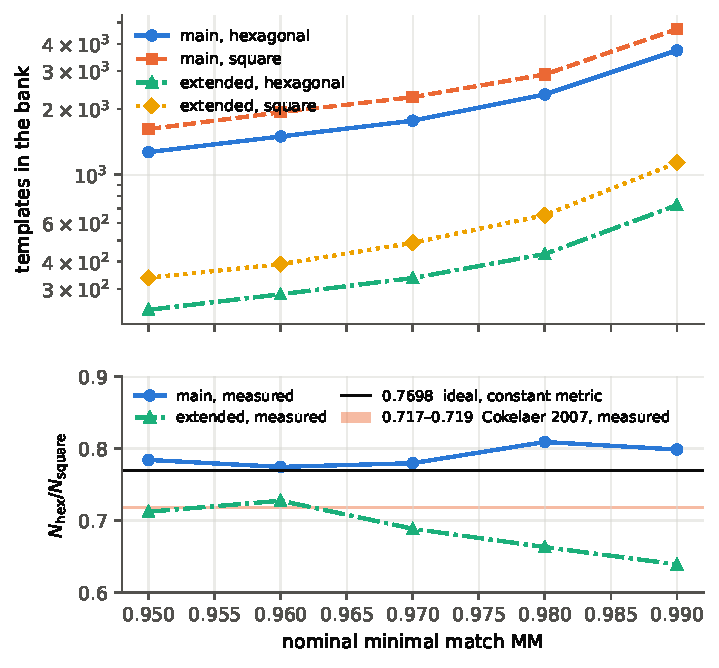
\includegraphics[width=0.62\textwidth]{d_counts_and_ratio.pdf}
\caption{Bank size and the measured ratio against its two references. \textbf{How this
could fail:} if lattice efficiency alone set the ratio, both regions would lie on one
horizontal line near $0.77$. They do not.}
\label{fig:counts}
\end{figure}

\begin{figure}[t]\centering
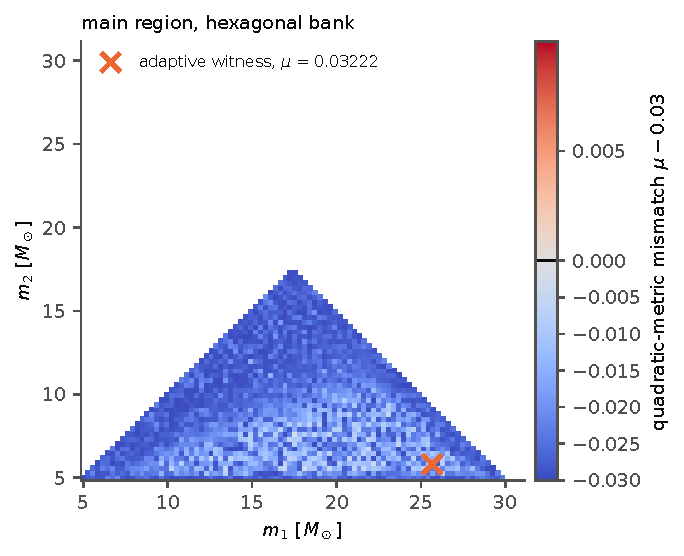
\includegraphics[width=0.56\textwidth]{d_mismatch_map_main_hex.pdf}
\caption{Mismatch to the nearest template over the mass plane, shown against both
component masses because the metric depends on both. \textbf{How this could fail:} a
covering bank would be uniformly below the target and none of this grid exceeds it --- yet
the marked point, found by an adaptive search, does. A figure built from grid sampling
alone would have shown a covering bank.}
\label{fig:map}
\end{figure}

\section{The threshold, and how many trials there really are}
\label{sec:results-threshold}

At the pre-registered operating point --- a false-alarm rate of $1/(100\,\mathrm{yr})$ over
one year --- solving $\mathrm{FAP} = 1 - (1-p)^{N}$ exactly with $p = e^{-\rho^2/2}$ gives
$\rho^* = \dataref{rho-star-naive-main-hexagonal}$ for the main hexagonal bank. The
rare-tail Poisson form agrees to $\dataref{poisson-approximation-error}$ relative, so the
approximation is safe --- shown rather than assumed.

Everything then depends on $N$. Counting every template and every sample as an independent
trial is an upper bound, and provably so: for a finite bank-and-time grid in centred
Gaussian noise the Gaussian correlation inequality gives
$\mathrm{FAP}(\rho) \le 1 - (1 - e^{-\rho^2/2})^{N}$. But it is a loose bound. Filtering
simulated noise through each bank and taking the maximum of $|z|$ over templates and time
gives $\nu_{\rm eff} = \dataref{nu-eff-main-hexagonal-mm097}$ independent trials per second
at $\MM = 0.97$, between six and seventeen times below the naive count --- and the gap
\emph{widens} with bank size.

That widening is the result. Fitting $N_{\rm eff} \propto N_{\rm templates}^{\alpha}$
within each family gives $\alpha = \dataref{trials-exponent-main-hexagonal}$ (main
hexagonal), $\dataref{trials-exponent-main-square}$, $\dataref{trials-exponent-extended-hexagonal}$
and $\dataref{trials-exponent-extended-square}$, every one of them more than eighteen
standard deviations below $1$. The mechanism is not subtle: refining a bank adds templates
that overlap their neighbours at the minimal match \emph{by construction}, so they add
redundancy, not independent trials.

\section{Volume, and the optimum that is not there}

Three losses must be kept apart, and Figure~\ref{fig:losses} keeps them apart: the exact
worst case $1 - \MM^3 = \dataref{worst-case-volume-loss-mm097}$, its linear expansion
$3(1-\MM)$, which is $3.06\,\%$ larger and is a different quantity, and the measured
population average. The last is
$\dataref{population-volume-loss-main-hexagonal-mm097}$ for the main hexagonal bank ---
\emph{four to nine times smaller than the worst case.} Almost no injection lands at the
worst point of its cell, so quoting $1 - \MM^3$ as what a bank costs overstates it by most
of an order of magnitude.

\begin{figure}[t]\centering
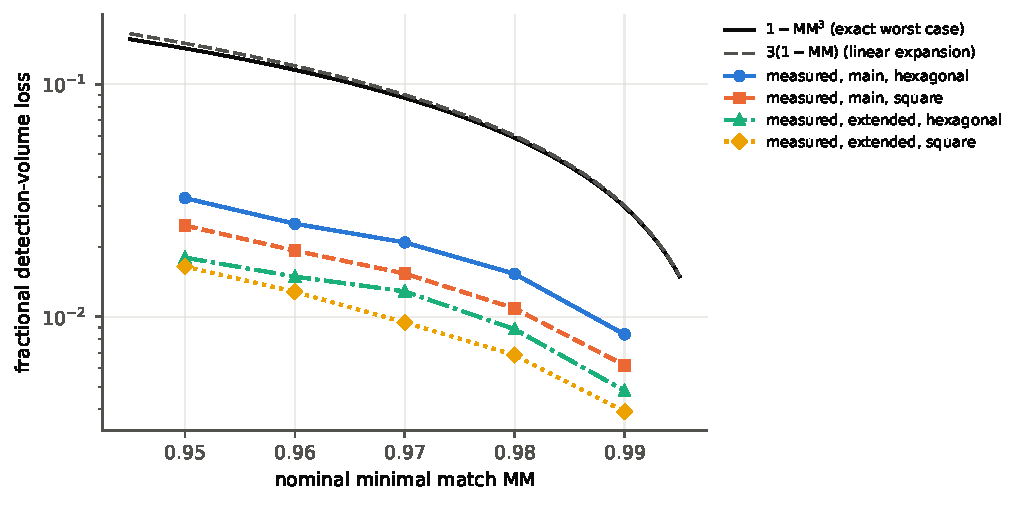
\includegraphics[width=0.70\textwidth]{f_volume_losses.pdf}
\caption{The three losses. \textbf{How this could fail:} if the worst case described what a
bank costs, the measured points would lie on the black curve.}
\label{fig:losses}
\end{figure}

The effective volume $V_{\rm eff} = \langle M^3\rangle / \rho^{*3}$ then answers whether
there is a best minimal match. Under the naive trials count it falls across
$\MM = 0.95$--$0.99$, by $\dataref{veff-change-naive-main-hexagonal}\,\%$ in the main
hexagonal case. Under the calibrated one it rises, by
$\dataref{veff-change-calibrated-main-hexagonal}\,\%$. The threshold is the reason:
calibrated, $\rho^*$ moves $0.24\,\%$ while the bank triples, against $1.46\,\%$ naive,
and the $2.48\,\%$ gain in $\langle M^3\rangle$ then wins.

\begin{figure}[t]\centering
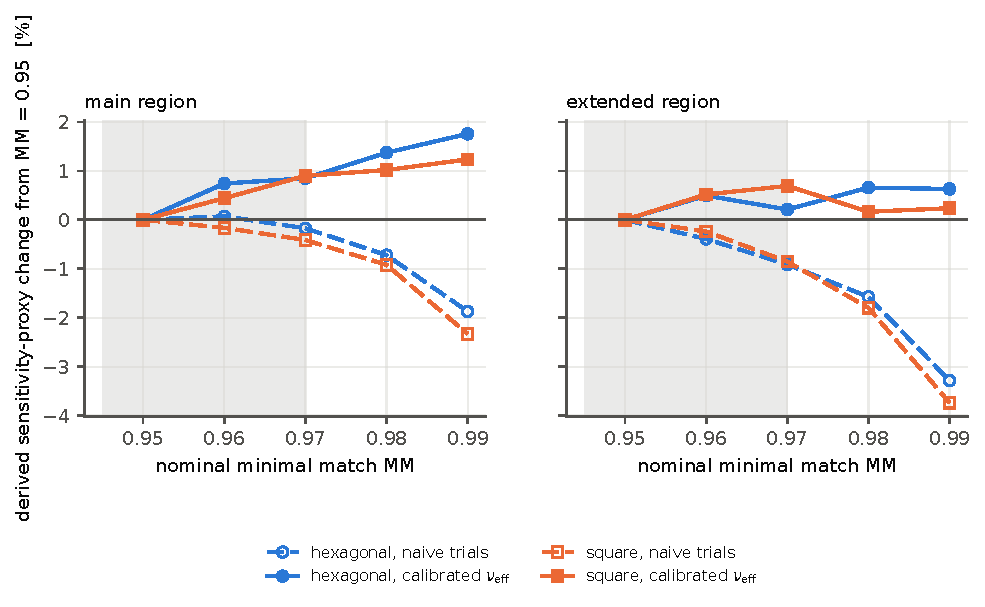
\includegraphics[width=0.90\textwidth]{f_veff_vs_mm.pdf}
\caption{Effective volume under both trials models. \textbf{How this could fail:} if the
two models agreed, the dashed and solid curves would coincide and the choice would not
matter.}
\label{fig:veff}
\end{figure}

Two things must be said about that reversal. The pre-registered hypothesis --- that the
threshold rise and the finer bank balance somewhere between $\MM = 0.97$ and $0.99$ --- is
not supported either way, but the calibrated curves are flat to within about $2\,\%$ and
are \emph{not} monotonic in the extended region, so no optimum is resolved inside the grid.
And the whole variation is smaller than the differences between the banks themselves. The
honest reading is that within this model the minimal match barely moves the effective
volume, and what weak preference exists is for finer banks. Where the optimum actually
sits is then fixed by computational cost --- the axis Keppel optimises, and the one this
work deliberately does not.

\section{What was not done}

\begin{itemize}\itemsep2pt
\item \textbf{No waveform check of the delivered banks.} Every covering number is the
      quadratic form. A sample of holes in an earlier bank was confirmed against real
      TaylorF2 matches, which found the quadratic form conservative rather than
      flattering, but none of the twenty banks reported here has been checked that way.
\item \textbf{Cokelaer's explicit connectors were never implemented.} Growth uses a
      proximity threshold as a stand-in, so the ``lattice only'' counts are not his
      lattice either.
\item \textbf{The pre-registered placement sensitivities were not run} --- a globally
      anchored metric, and discarding non-physical cells rather than projecting them.
\item \textbf{$\nu_{\rm eff}$ was calibrated at one segment length}, and extrapolated to a
      year as a rate. A half-segment check gives $0.432$ against an expected $0.5$.
\item \textbf{The IMRPhenomD volume leg is an approximation}, composing a continuous-family
      fitting factor with the discretisation match and assuming the two are independent.
      The rigorous statement is the family-only bound, which is quoted beside it.
\item \textbf{An independent cross-check of bank spacing by SVD} was planned and cut.
\end{itemize}

\section{Conclusion}

The two questions this work set out to answer have asymmetric answers. How much SNR a
mismatch costs is exact and settled: the loss is the mismatch, and above $M = 35\,\Msun$
the dominant loss is not the bank at all but the waveform model, at half the detection
volume. How dense a bank must be has no answer in these terms, because within a plausible
range the effective volume hardly depends on the density, and the direction of what little
dependence there is turned out to be set by the trials model rather than by the bank. The
practical content of the second answer is therefore negative, and worth stating plainly:
the minimal match is not where the sensitivity of this search is won or lost.

\paragraph{Reproducing this.} Every number above resolves through \verb|\dataref| against
\verb|data/project_numbers.json|, whose sole writer is \verb|scripts/compute_numbers.py|;
every figure is produced by \verb|scripts/make_figures.py| and by nothing else, from the
tracked data in \verb|data/|. \verb|tests/test_acceptance.py| pins the reported values.

\end{document}
